\documentclass{beamer}
\usepackage{tikz}
\usepackage{tikz-qtree}
\usepackage{gillius}
\usepackage{mathdots}
\usepackage{abraces}
\usepackage{etex}
\usepackage{array}
\usepackage[backend=biber]{biblatex}

% http://tex.stackexchange.com/questions/12703/how-to-create-fixed-width-table-columns-with-text-raggedright-centered-raggedlef
\newcolumntype{L}[1]{>{\raggedright\let\newline\\\arraybackslash\hspace{0pt}}m{#1}}
\newcolumntype{C}[1]{>{\centering\let\newline\\\arraybackslash\hspace{0pt}}m{#1}}
\newcolumntype{R}[1]{>{\raggedleft\let\newline\\\arraybackslash\hspace{0pt}}m{#1}}

\usetikzlibrary{external}
\usetikzlibrary{shapes}
\usetikzlibrary{arrows}
\usetikzlibrary{positioning}
\usetikzlibrary{decorations.pathreplacing}

\usetheme[everytitleformat=regular]{m}
\setbeamertemplate{navigation symbols}{}

\title{M.Sc. Thesis Proposal: Phylodynamic Inference of Contact Network
Structures with Approximate Bayesian Computation}
\author[RM \& AFYP]{Rosemary McCloskey and Art FY Poon}
\institute[UBC \& BCCfE]{BC Centre for Excellence in HIV/AIDS \\ University of British Columbia}
\date{September 22, 2015}

\newcommand{\dd}[2]{\frac{\text{d}\,#1}{\text{d}\,#2}}

\begin{document}
\definecolor{red}{RGB}{228,26,28}
\definecolor{blue}{RGB}{55,126,184}
\definecolor{green}{RGB}{77,175,74}
\definecolor{purple}{RGB}{152,78,163}

\maketitle
\begin{frame}{Outline}
    \begin{enumerate}
        \setlength{\itemsep}{12pt}
        \item Motivation
        \item Proposed methods
        \item Proof of concept
        \item Rotation project: phylogenetic clustering
    \end{enumerate}
\end{frame}

\section{Motivation}

\begin{frame}{Phylodynamics}
    \vspace{-1cm}
    \begin{center}
    \begin{tikzpicture}
        \uncover<1-2>{
        \node (a) {\includegraphics[width=1cm]{hiv}};
        \node at (a.north west) {\includegraphics[width=1cm]{person2}};
        }\uncover<2>{
        \node [right=1.5cm of a] (b) {\includegraphics[width=1cm]{hiv}};
        \node at (b.north west) {\includegraphics[width=1cm]{person1}};
        }
        
        \uncover<3->{
        \node [right=1.5cm of a, opacity=0.4] (b) {\includegraphics[width=1cm]{hiv}};
        \node at (b.north west) [opacity=0.4] {\includegraphics[width=1cm]{person1}};
        \node (a) [opacity=0.4] {\includegraphics[width=1cm]{hiv}};
        \node at (a.north west) [opacity=0.4] {\includegraphics[width=1cm]{person2}};
        }
        
        
        \uncover<2-3>{
        \draw[->, >=stealth, thick] (a) -- (b);
        }\uncover<3->{
        \node [below=2cm of a] (c) {\includegraphics[width=1cm]{hiv}};
        \node at (c.north west) {\includegraphics[width=1cm]{person2}};
        \node [below=2cm of b] (d) {\includegraphics[width=1cm]{hiv}};
        \node at (d.north west) {\includegraphics[width=1cm]{person1}};
        }\uncover<3->{
        \coordinate [left= of a] (timestart);
        \coordinate [left= of c] (timeend);
        \draw[->, >=stealth, thick] (timestart) -- node[auto, swap] {time} (timeend);
        }\uncover<4->{
        \coordinate [right=1.4 of a.center] (root);
        \draw [very thick] (a.center) +(1.4, 0) to +(1.4, 1);
        \draw [very thick] (c.center) -- (root);
        \draw [very thick] (d.center) -- (root);
        \draw [very thick] (root) to +(0, 1);
        }

        \uncover<2->{
        \node (note1) [right= of b, text width=4.5cm] {transmission to new host \\
        $\Rightarrow$ isolated sub-population};
        }
        \uncover<3->{
            \node (note2) [below=0.8cm of note1, text width=4.5 cm] {within-host evolution};
        }
        \uncover<4->{
            \node [below=of note2, text width=4.5 cm] {virus phylogeny \\ $\approx$ transmission tree};
        }
    \end{tikzpicture}
\end{center}
\end{frame}

\begin{frame}{State-of-the-art: population-level parameters}
    \begin{columns}
        \begin{column}{0.5\textwidth}
            \includegraphics[width=\textwidth]{cumulative}
        \end{column}
        \begin{column}{0.5\textwidth}
            \includegraphics[width=\textwidth]{tmrca}
        \end{column}
    \end{columns}
    \begin{columns}
        \begin{column}{0.5\textwidth}
            \tiny{Volz, Erik, and Sergei Pond. ``Phylodynamic analysis of Ebola virus in the 2014 Sierra Leone epidemic.'' PLoS currents 6 (2014).}
        \end{column}
        \begin{column}{0.5\textwidth}
            \tiny{Liao, Huanan, et al. ``Phylodynamic analysis of the dissemination of HIV-1 CRF01\_AE in Vietnam.'' Virology 391.1 (2009): 51-56.}
        \end{column}
    \end{columns}
\end{frame}

\begin{frame}{Network structure profoundly affects tree shape}

    \includegraphics[trim=0 -1cm 0 0]{odea-f2a}\includegraphics{odea-f2d}

    \begin{center}
    ``Contact heterogeneity is well known to have a strong effect on infectious
    disease dynamics. We have shown how the relationship between infectious
    disease dynamics and genealogies is similarly sensitive to the contact
    heterogeneity specified by a network.''
    
    \tiny{O'Dea, Eamon B., and Claus O. Wilke. ``Contact heterogeneity and
        phylodynamics: how contact networks shape parasite evolutionary
        trees.'' Interdisciplinary Perspectives on Infectious Diseases 2011
    (2010).}
    \end{center}
\end{frame}

\begin{frame}{Research question}
    \large
    \begin{enumerate}
        \setlength{\itemsep}{12pt}
        \item Are there contact network parameters which are possible to infer
            with phylogenetic methods?
        \pause
        \item What are the estimated values of those parameters for the HIV
            subtype B-infected population in British Columbia?
    \end{enumerate}
\end{frame}

\section{Proposed Methods}

\begin{frame}{Approximate Bayesian computation}
    \begin{tabular}{C{4cm}C{3cm}C{2cm}}
        goal & & data \\
        \hline\\
        $N$ = number of people, \newline $k$ = average number of partners & &
        \includegraphics[scale=0.5]{tree2.pdf} \\
        \\ \hline \\
        \uncover<2->{$N = 1000, k = 3$} & 
        \uncover<3->{\includegraphics[scale=0.5]{net1.pdf}} &
        \uncover<4->{\includegraphics[scale=0.5]{tree1.pdf}} \\
        \uncover<5->{$N = 1000, k = 12$} & 
        \uncover<6->{\includegraphics[scale=0.5]{net2.pdf}} &
        \uncover<7->{\includegraphics[scale=0.5]{tree3.pdf}} \\
    \end{tabular}
\end{frame}

\begin{frame}{Approximate Bayesian computation}
    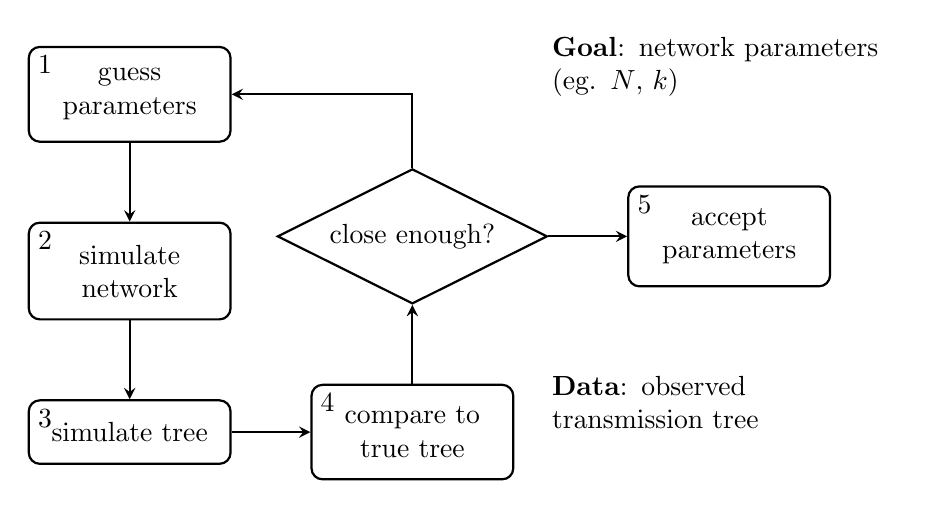
\begin{tikzpicture}
        [state/.style={rounded corners, rectangle, draw, inner sep=8pt, text width=2cm, align=center},
        decision/.style={diamond, aspect=2, draw},
        every path/.style={->, >=stealth, thick}]
        \node[state] (1) {guess parameters};
        \node[state, below=of 1] (2) {simulate network};
        \node[state, below=of 2] (3) {simulate tree};
        \node[state, right=of 3] (4) {compare to true tree};
        \node[decision, above=of 4] (5) {close enough?};
        \node[state, right=of 5] (6) {accept parameters};
        \node[above=of 6, text width=4.5cm] {\textbf{Goal}: network parameters \newline (eg. $N$, $k$)};
        \node[below=of 6, text width=4.5cm] {\textbf{Data}: observed \newline transmission tree};
        \node at (1.north west) [anchor=north west] {1};
        \node at (2.north west) [anchor=north west] {2};
        \node at (3.north west) [anchor=north west] {3};
        \node at (4.north west) [anchor=north west] {4};
        \node at (6.north west) [anchor=north west] {5};
        \draw (1) -- (2);
        \draw (2) -- (3);
        \draw (3) -- (4);
        \draw (4) -- (5);
        \draw (5.north) |- (1);
        \draw (5) -- (6);
    \end{tikzpicture}
\end{frame}

\begin{frame}{Plan}
    Data: phylogeny of $\sim$8000 HIV infections in BC.
    \begin{enumerate}
        \item[0.] Literature review.
        \item Guess parameters: preliminary experiments to determine which
            parameters are identifiable.
        \pause
        \item Simulate network: out-of-the-box, possibly exponential random
            graph model (ERGM).
        \pause
        \item Simulate tree: next-reaction method (already done).
        \pause
        \item Compare to true tree: Art's tree kernel.
        \pause
        \item ABC algorithm: sequential Monte-Carlo or Markov chain Monte Carlo.
    \end{enumerate}
\end{frame}

\section{Proof of Concept}

\begin{frame}{Verifying tree simulations}
    Leventhal et al: Sackin's index for simulated phylogenies over networks of
    5000 nodes.
    \begin{center}
    \includegraphics[scale=1.5, trim=0 0 3.5cm 0, clip=true]{f1}
    \uncover<2->{\includegraphics[scale=0.07]{sackin}}
    \end{center}

    \tiny{Leventhal, Gabriel E., et al. ``Inferring epidemic contact structure from phylogenetic trees.'' PLoS Comput Biol 8.3 (2012)}
\end{frame}

\begin{frame}{Kernel matrices of simulated trees}
    \includegraphics[scale=0.3]{kmat5k}
    \includegraphics[scale=0.3]{kmat100}

    $\qquad$$\qquad$ 5000 nodes \hfill 100 nodes $\qquad$$\qquad$$\quad$
\end{frame}

\begin{frame}{Aside: clustering}
    \includegraphics[trim=1in 0 0 4in, clip=true]{f3a}
    \includegraphics[scale=0.7]{f3b}

    \tiny{Lewis, Fraser, et al. ``Episodic sexual transmission of HIV revealed by molecular phylodynamics.'' PLoS Med 5.3 (2008).}
\end{frame}

\begin{frame}{Aside: clustering}
    \begin{columns}
        \begin{column}{0.5\textwidth}
            \includegraphics[width=\textwidth]{ba-net}
        \end{column}
        \begin{column}{0.5\textwidth}
            \includegraphics[width=\textwidth]{ba-tree}
        \end{column}
    \end{columns}
\end{frame}

\section{Rotation Project: Phylogenetic Clustering}

\begin{frame}{Clustering by Branching Rates}
    \only<1>{\includegraphics[height=\textwidth,angle=-90]{pcbr_example}}
    \only<2->{\includegraphics[height=\textwidth,angle=-90]{pcbr_example_color}}

    \hspace{1.2cm}
    \uncover<3->{
    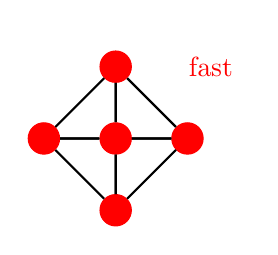
\begin{tikzpicture}
        [node distance=0.5,
         every node/.style={circle, draw=red, fill=red, inner sep=4pt}]
        \node (a) { };
        \node [below=of a] (b) { };
        \node [below=of b] (c) { };
        \node [right=of b] (d) { };
        \node [left=of b] (e) { };
        \draw [thick] (a) -- (b) -- (d) -- (a);
        \draw [thick] (a) -- (b) -- (e) -- (a);
        \draw [thick] (c) -- (b) -- (d) -- (c);
        \draw [thick] (c) -- (b) -- (e) -- (c);
        \node [right=of a, draw=none, fill=none, text=red] {fast};
    \end{tikzpicture}
    }
    \hspace{0.2cm}
    \uncover<4->{
    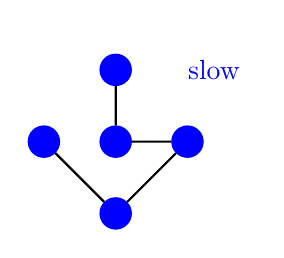
\begin{tikzpicture}
        [node distance=0.5,
         every node/.style={circle, draw=blue, fill=blue, inner sep=4pt}]
        \node (a) { };
        \node [below=of a] (b) { };
        \node [below=of b] (c) { };
        \node [right=of b] (d) { };
        \node [left=of b] (e) { };
        \draw [thick] (a) -- (b) -- (d) -- (c) -- (e);
        \node [right=of a, draw=none, fill=none, text=blue] {slow};
    \end{tikzpicture}
    }
\end{frame}

\begin{frame}{Modelling branching rates}
    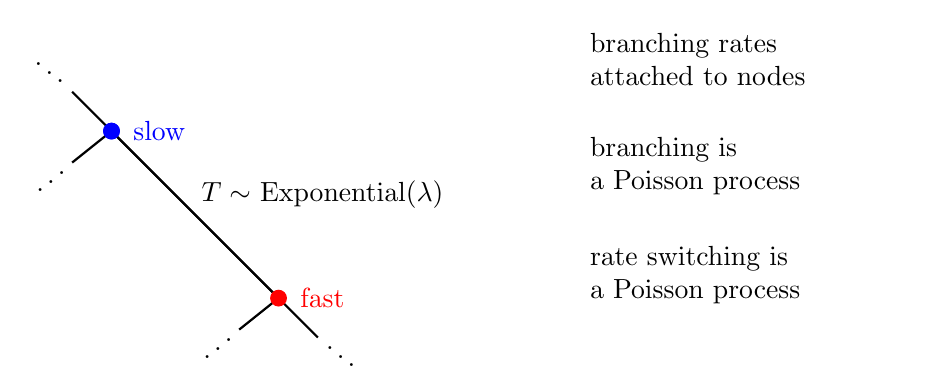
\begin{tikzpicture}
        [every node/.style={inner sep=2pt}]
        \coordinate (a);
        \coordinate [below right=3 of a] (b);
        \draw [thick] (a) -- ++ (-0.5, 0.5) node [anchor=south east] {$\ddots$};
        \draw [thick] (a) -- ++ (-0.5, -0.4) node [inner ysep=-4pt, inner xsep=2pt, anchor=north east] {$\iddots$};
        \draw [thick] (b) -- ++ (-0.5, -0.4) node [inner ysep=-4pt, inner xsep=2pt, anchor=north east] {$\iddots$};
        \draw [thick] (b) -- ++ (0.5, -0.5) node [anchor=north west, inner ysep=-4pt] {$\ddots$};
        \draw [thick] (a) -- (b);
        \uncover<2->{
            \node at (a) [circle, draw=blue, fill=blue] { };
            \node [right=0.2 of a, anchor=west, text=blue] {slow};
            \node (note1) [above right=0.5 and 6 of a, text width=4cm] {branching rates \\ attached to nodes};
        }
        \uncover<3->{
            \draw [thick] (a) -- node [auto] {
                $T \sim $ Exponential($\lambda$)
            } (b);
            \node at (a) [circle, draw=blue, fill=blue] { };
            \node (note2) [below=0.5 of note1, text width=4cm] {branching is \\ a Poisson process};
        }
        \uncover<4->{
            \node at (b) [circle, draw=red, fill=red] { };
            \node [right=0.2 of b, anchor=west, text=red] {fast};
            \node [below=0.5 of note2, text width=4cm] {rate switching is \\ a Poisson process};
        }
    \end{tikzpicture}

    \begin{center}
    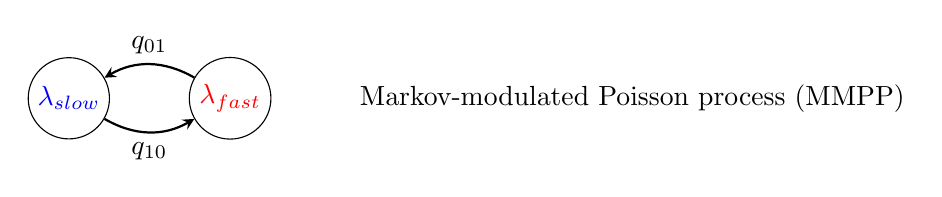
\begin{tikzpicture}
    \uncover<5->{
        \node [circle, draw, text=blue, inner sep=2pt] (slow) {$\lambda_{\text{slow}}$};
        \node [right=of slow, circle, draw, text=red, inner sep=2pt] (fast) {$\lambda_{\text{fast}}$};
        \draw [->, >=stealth, thick] (slow) to [bend right] node[auto, swap] {$q_{10}$} (fast);
        \draw [->, >=stealth, thick] (fast) to [bend right] node[auto, swap] {$q_{01}$} (slow);
    }
    \uncover<6->{
        \node [right=of fast] {Markov-modulated Poisson process (MMPP)};
    }
    \end{tikzpicture}
    \end{center}
\end{frame}

\begin{frame}{Validation}
    Works fairly well for superspreader networks.
    \vspace{0.5cm}
    \begin{columns}
        \begin{column}{0.5\textwidth}
            \includegraphics[width=\textwidth]{stadler2}
        \end{column}
        \begin{column}{0.5\textwidth}
            \includegraphics[width=\textwidth]{2_2_008}
        \end{column}
    \end{columns}
\end{frame}

\begin{frame}{Validation}
    Doesn't work for interconnected islands model.
    \vspace{0.5cm}
    \begin{columns}
        \begin{column}{0.5\textwidth}
            \includegraphics[width=\textwidth]{stadler1}
        \end{column}
        \begin{column}{0.5\textwidth}
            \includegraphics[width=\textwidth]{1_2_197}
        \end{column}
    \end{columns}
\end{frame}

\begin{frame}{Validation}
    Doesn't work well for scale-free networks (hard to define ``true'' clusters).
    \vspace{0.5cm}
    \begin{columns}
        \begin{column}{0.5\textwidth}
            \includegraphics[width=\textwidth]{stadler3}
        \end{column}
        \begin{column}{0.5\textwidth}
            \includegraphics[width=\textwidth]{3_3_072}
        \end{column}
    \end{columns}
\end{frame}

\begin{frame}{Validation}
    No clusters detected with differential risk trees.

    \vspace{0.5cm}
    \begin{center}
    \includegraphics[scale=0.44445]{diffrisk}
    \end{center}
\end{frame}

\begin{frame}
    \begin{center}
    \Huge{Thank you!}
    \end{center}
\end{frame}

\end{document}
